%!TEX root=../../root.tex

Until now we have seen examples in 1 or 2 dimensions but in practice we will often deal with higher dimensional cases, like images.

Consider a greyscale image (each pixel value is $\in [0, 1]$), of width $w$ and height $h$, it will have a total of $wh$ dimensions;
this image can be considered a point in a $wh$-dimensional space.
A dataset of such images is a point cloud in $\mathbb{R}^{wh}$.

\smallskip
\begin{center}
	\begin{overpic}
	    [trim=0cm 0cm 0cm 0cm,clip,width=0.35\linewidth]{02/yokohama}
	    \put(105,32){$\in\mathbb{R}^{w\times h} \cong \mathbb{R}^{wh}$}
	\end{overpic}
\end{center}
\smallskip
For example, a $\sim$1 megapixel photo (grayscale) has $\sim 10^6$ dimensions.
Often, the question to ask is whether all these dimensions are significant.

Let's now delve into an explanation of the so-called \emph{curse of dimensionality};
for simplicity, consider $1 \shorttimes 1$ images consisting of one single pixel. Since there is only one dimension, we can put all these images along 
the real axis, sorting them by value. 

\begin{figure}[H]
	\centering
	
\includegraphics[width=.5\textwidth]{02/dim1}
	\caption{$1 \shorttimes 1$ images on the real axis.}\label{fig:1x1imgs}	
\end{figure}

Now consider $2 \shorttimes 1$ images, and place them as points in the 2-dimensional space with respect to their value.

\begin{figure}[H]
	\centering
	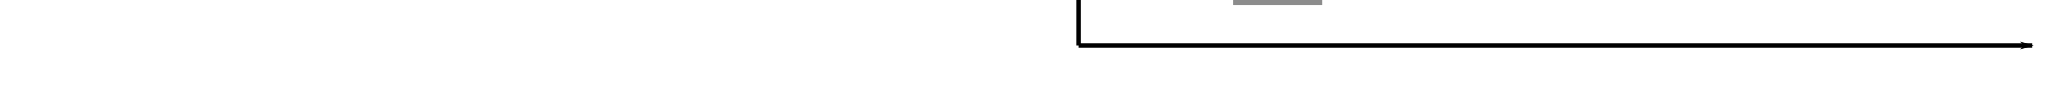
\includegraphics[width=.5\textwidth]{02/dim2}
	\caption{$2 \times 1$ images on the real axis.}\label{fig:2x1imgs}	
\end{figure}

If we do this for $3 \shorttimes 1$ images, we can see that as the dimensionality grows,
the points in the space become more and more sparse; increasing dimension increases the sparsity of the point cloud.

\begin{figure}[H]
	\centering
	\includegraphics[width=.5\textwidth]{02/dim3}
	\caption{$3 \shorttimes 1$ images on the real axis.}\label{fig:3x1imgs}	
\end{figure}

A dataset of natural images will be extremely sparse in $\mathbb{R}^{wh}$, since
each region of the ambient space will be observed very infrequently, expecially if we have few images.
As we add new images, each one will not be very likely to fall close to the previous one.
It can be proved that as we increase dimensionalities all points (each point is an image of the dataset) will eventually become equally spaced from the others. 

If our dataset consists of equally spaced points, no meaningful structure will emerge from the dataset, and therefore there won't be anything interesting to learn about it.
We would need to increase the number of data points (so the images of the dataset) exponentially in the number of dimensions. 
If $n$ data points cover well the space of $1$-dimensional images, then $n^d$ data points are required for $d$-dimensional images.

\subsection{Decrease the dimensions}

\subsubsection{Features}
Assume each data point $x \in \mathcal{D} \subset \mathbb{R}^n$ is the result of a synthesis, or generation, process:
\begin{equation}
    \sigma : F \rightarrow x
\end{equation}
which takes a set of features $F$ and composes them to form $x$. Deep learning is about discovering $F$ from $x$ and simultaneously discovering $\sigma$.

\begin{ex}
An image $x\in\mathbb{R}^{w\times h}$ is composed by pixels. 

\smallskip

If each pixel of $x$ is a feature, then $\sigma$ simply sums them up:

\medskip

\begin{center}
	\begin{overpic}[trim=0cm 0cm 0cm 0cm,clip,width=0.8\linewidth]{02/yokohama_lin}
		\put(19,8){\footnotesize $=\alpha_1$}
		\put(46.5,8){\footnotesize $+\alpha_2$}
		\put(74,8){\footnotesize $+\alpha_3$}
		\put(100.5,8){\footnotesize $+\cdots$}
	\end{overpic}
\end{center}
In this case, the \emph{feature space} $F$ is spanned by individual pixels. Each feature (each pixel) represents a dimension.
This can be expressed concisely as
\begin{equation}
	x = \sigma(F) = \sum_{f_i\in F} \alpha_i \cdot f_i
\end{equation}
where $\alpha_i$ are the \emph{weights} in the representation of $x$.
In this \textbf{particular case}, the feature space is a \emph{vector space} and $\sigma$ is \emph{linear}.
\end{ex}


Having one feature per pixel is extremely wasteful; in general, the curse of dimensionality occurs when

\begin{center}
	\emph{features} $\gg$ \emph{observations}
\end{center}

\medskip
In cases like this, we may want to find a different representation which doesn't fall in the curse of dimensionality, so we are basically asking what really characterizes our image.

\begin{ex} 
	The following image may be represented as a combination of these three features:

	\smallskip

	\begin{center}
			\begin{overpic}[trim=0cm 0cm 0cm 0cm,clip,width=0.6\linewidth]{02/yokohama_nonlin}
			\put(28,10){\Large $=\sigma($}
			\put(69,10){\Large $,$}
			\put(81,10){\Large $,$}
	      	\put(103,10){\Large $)$}
			\end{overpic}
	\end{center}

	or we may try to use even fewer features: the image may be represented using the first square, representing the white square as a modified version of the black box with different size and color and the black line as a degenere case. 
\end{ex}

In general, the transformation $\sigma$ acts \emph{nonlinearly} on the features. The output of $\sigma$ is called an \emph{embedding} of the data point.
For the data point $x\in \mathcal{D} \subset \mathbb{R}^n$, the \emph{embedding space} is $\mathbb{R}^n$.

What we are actually doing is not getting rid of the complexity, but hiding it in $\sigma$.

In deep learning, $\sigma$ will be a deep neural network and the features will be the intermediate representation of the image; a trade-off between the number of features and the complexity of $\sigma$ must be decided.

\paragraph{Intrinsic invariances}
In general, a given data point admits many possible embeddings.
\begin{ex}
	A sheet lives naturally in $\mathbb{R}^2$, but is usually embedded in $\mathbb{R}^3$.

	\begin{figure}[H]
		\begin{center}
			\begin{overpic}[trim=0cm 0cm 0cm 0cm,clip,width=0.2\linewidth]
				{02/sheet1}
			\end{overpic}
			\begin{overpic}[trim=0cm 0cm 0cm 0cm,clip,width=0.5\linewidth]
				{02/sheet2}
			\end{overpic}
		\end{center}
		\caption{Three different embeddings of the same object.}
	\end{figure}
	Even if the embeddings look totally different, distances are preserved in all of them.
\end{ex}

In general, the challenge will be to discover what \emph{intrinsic} properties are preserved; these properties characterize the data.

\paragraph{Latent features}
In the general case:

\begin{itemize}
	\item features are not necessarily \emph{localized} in space, and
	\item features are not necessarily \emph{evident} in the embedding.
\end{itemize}

We thus talk about \emph{latent} features, which are characterizing properties of the image that are hidden; more examples may be necessary to extract this kind of features. The problem is that we only have direct access to the embedding.

\begin{ex}
	It is obvious for an human that the only difference among the various images in \cref{fig:lights} is that the light source is moving around the face. However, this is may not be obvious for a learning model. Let's say we want to design a model which, taken an image, relights it from different positions. The model can be parametrized with only 4 parameters, $(x,y,z)$ for the light position and maybe another parameter for the intensity. 
	\begin{figure}[H]
		\centering
		\includegraphics[width=\textwidth]{02/lights}
		\caption{Example of a latent feature: directional illumination.}\label{fig:lights}	
	\end{figure}
\end{ex}

In general, discovering latent features involves discovering:
\begin{itemize}
	\item the ``true'' embedding space for the data, and
	\item the \emph{transformation} between the two spaces.
\end{itemize}

We would like to discard the \emph{non-informative} dimensions from the data.

\paragraph{Dimensionality}

Even just discovering the intrinsic dimensionality is a challenge by itself. Usually, it is specified by hand by whoever designs the learning model. 
In \cref{fig:hughes} we can see a representation of the Hughes phenomenon; in the original experiment, a classification model was trained with different intrinsic dimensionalities ($x$ axis) and the accuracy was recorded for each of these ($y$ axis); each curve in the plot represents a dataset. 
As you can see, every curve reaches a local maximum with a certain dimensionality and then sees its accuracy decrease as the dimensionality gets bigger and bigger. 

\begin{figure}[H]
	\centering
	\includegraphics[width=.5\textwidth]{02/hughes}
	\caption{The Hughes phenomenon.}\label{fig:hughes}	
\end{figure}

Finding a lower-dimensional embedding for some given data is a dimensionality reduction problem. Usually, this is done by nonlinear dimensionality reduction techniques.

\begin{figure}[H]
	\centering
	\includegraphics[width=.5\textwidth]{02/roll}
	\caption{Swiss roll plot.}\label{fig:roll}	
\end{figure}

This class of problems is also called \emph{manifold learning}. However it must not be confused with deep learning; the former only finds a lower-dimensional embedding for the data, while the latter finds patterns in the data, and also determines a map.

In deep learning the \emph{manifold hypothesis} is assumed to hold; that is, the input data is assumed to live on some underlying non-Euclidean structure called a manifold.

\begin{defn}[Manifold]
	A manifold is a topological space that locally resembles Euclidean space near each point. More precisely, an $n$-dimensional manifold is a topological space with the property that each point has a neighborhood that is homeomorphic to the Euclidean space of dimension $n$.
\end{defn}

\begin{figure}[H]
 	\centering
 	\includegraphics[width=.5\textwidth]{02/manifold}
 	\caption{A manifold.}\label{fig:manifold}	
 \end{figure} 

\paragraph{Task-driven features}
Speaking about features only makes sense if we are given a task to solve, for example, color in a deck of french cards is important only in some card games.

We are now ready to give a more comprehensive definition of deep learning.

\begin{defn}[Deep learning]
	Deep learning is a task-driven paradigm to extract patterns and latent features from given observations.
\end{defn}

It must be said nevertheless that features are not always the focus of deep learning; rather, they are usually instrumental for the given task.
